\section{Introduction}
\label{sec:intro}

%\yu{What's online shopping assistant?}
An intelligent online shopping assistant
offers services such as pre-sale and after-sale inquiries, 
product recommendations, and user complaints processing,
all of which seek to give the customers better shopping experience.
%\figref{fig:dialog-case} shows an example snapshot of 
%such a shopping assistant. 
%%\KZ{This figure is not effective. Too messy and not intuitive. I suggest we cut it. Just show a simple interface with a short conversation.}
%It is a dialog module embedded in operational Taobao product search engine 
%and serves as a shopping assistant on mobile Taobao.
%In this example, a customer wants to buy a dress firstly. 
%Then the assistant helps him
%narrow down the search by getting information such as 
%(\textbf{Brand}=Nike, \textbf{Color}=black).
%Finally the customer changes his mind and wants to buy milk powder instead,
%and this will start the next round of conversation.
%\KZ{Rephrase the following...}
%In addition to this, our system also responds to product queries. 
%All of these aim to help customers find and buy the products of their choice
%in a friendly and efficient way.
%\begin{figure*}[th]
%	\centering
%	\epsfig{file=figures/dialog_case.eps, width=2.0\columnwidth}
%	\caption{An example snapshot of online E-commerce shopping assistant.
%	Customers will interact with our system and give sequential utterances to refine their information need or change the product intent.}
%	\label{fig:dialog-case}
%	\vspace{-10pt}
%\end{figure*}
%\yu{2. Dialog system, conversational search and slot filling}
The core of such assistant is a task-oriented dialog system which 
has the ability to understand natural language utterances
from a user and then give natural language responses \cite{yan2017building}.
%The general framework of such a task-oriented dialog system
%is illustrated in \figref{fig:dialog-system}.
%Besides modules of dialog management (DM) and 
%natural language generation (NLG),
%the very fist step of a dialog system is
%The difference between this and a traditional task-oriented dialog systems
%is that it interacts with a product search engine.
%So we can also regard it as an E-commerce conversational search system.
Natural Language Understanding (NLU), which aims to 
interpret the semantic meanings conveyed by input utterances, 
is a main component in task-oriented dialog systems. 
%Slot filling is a sub-problem in NLU, which identifies
%the properties and their values about the task to be performed in the dialog.
%\yu{In our E-commerce shopping guide assistant system, slot filling is not only helpful for Dialog State Tracking but also for Query Rewrite.}
%\xusheng{mentioning DST and query rewrite is a little bit strange here}
%\begin{figure}[th]
%	\centering
%	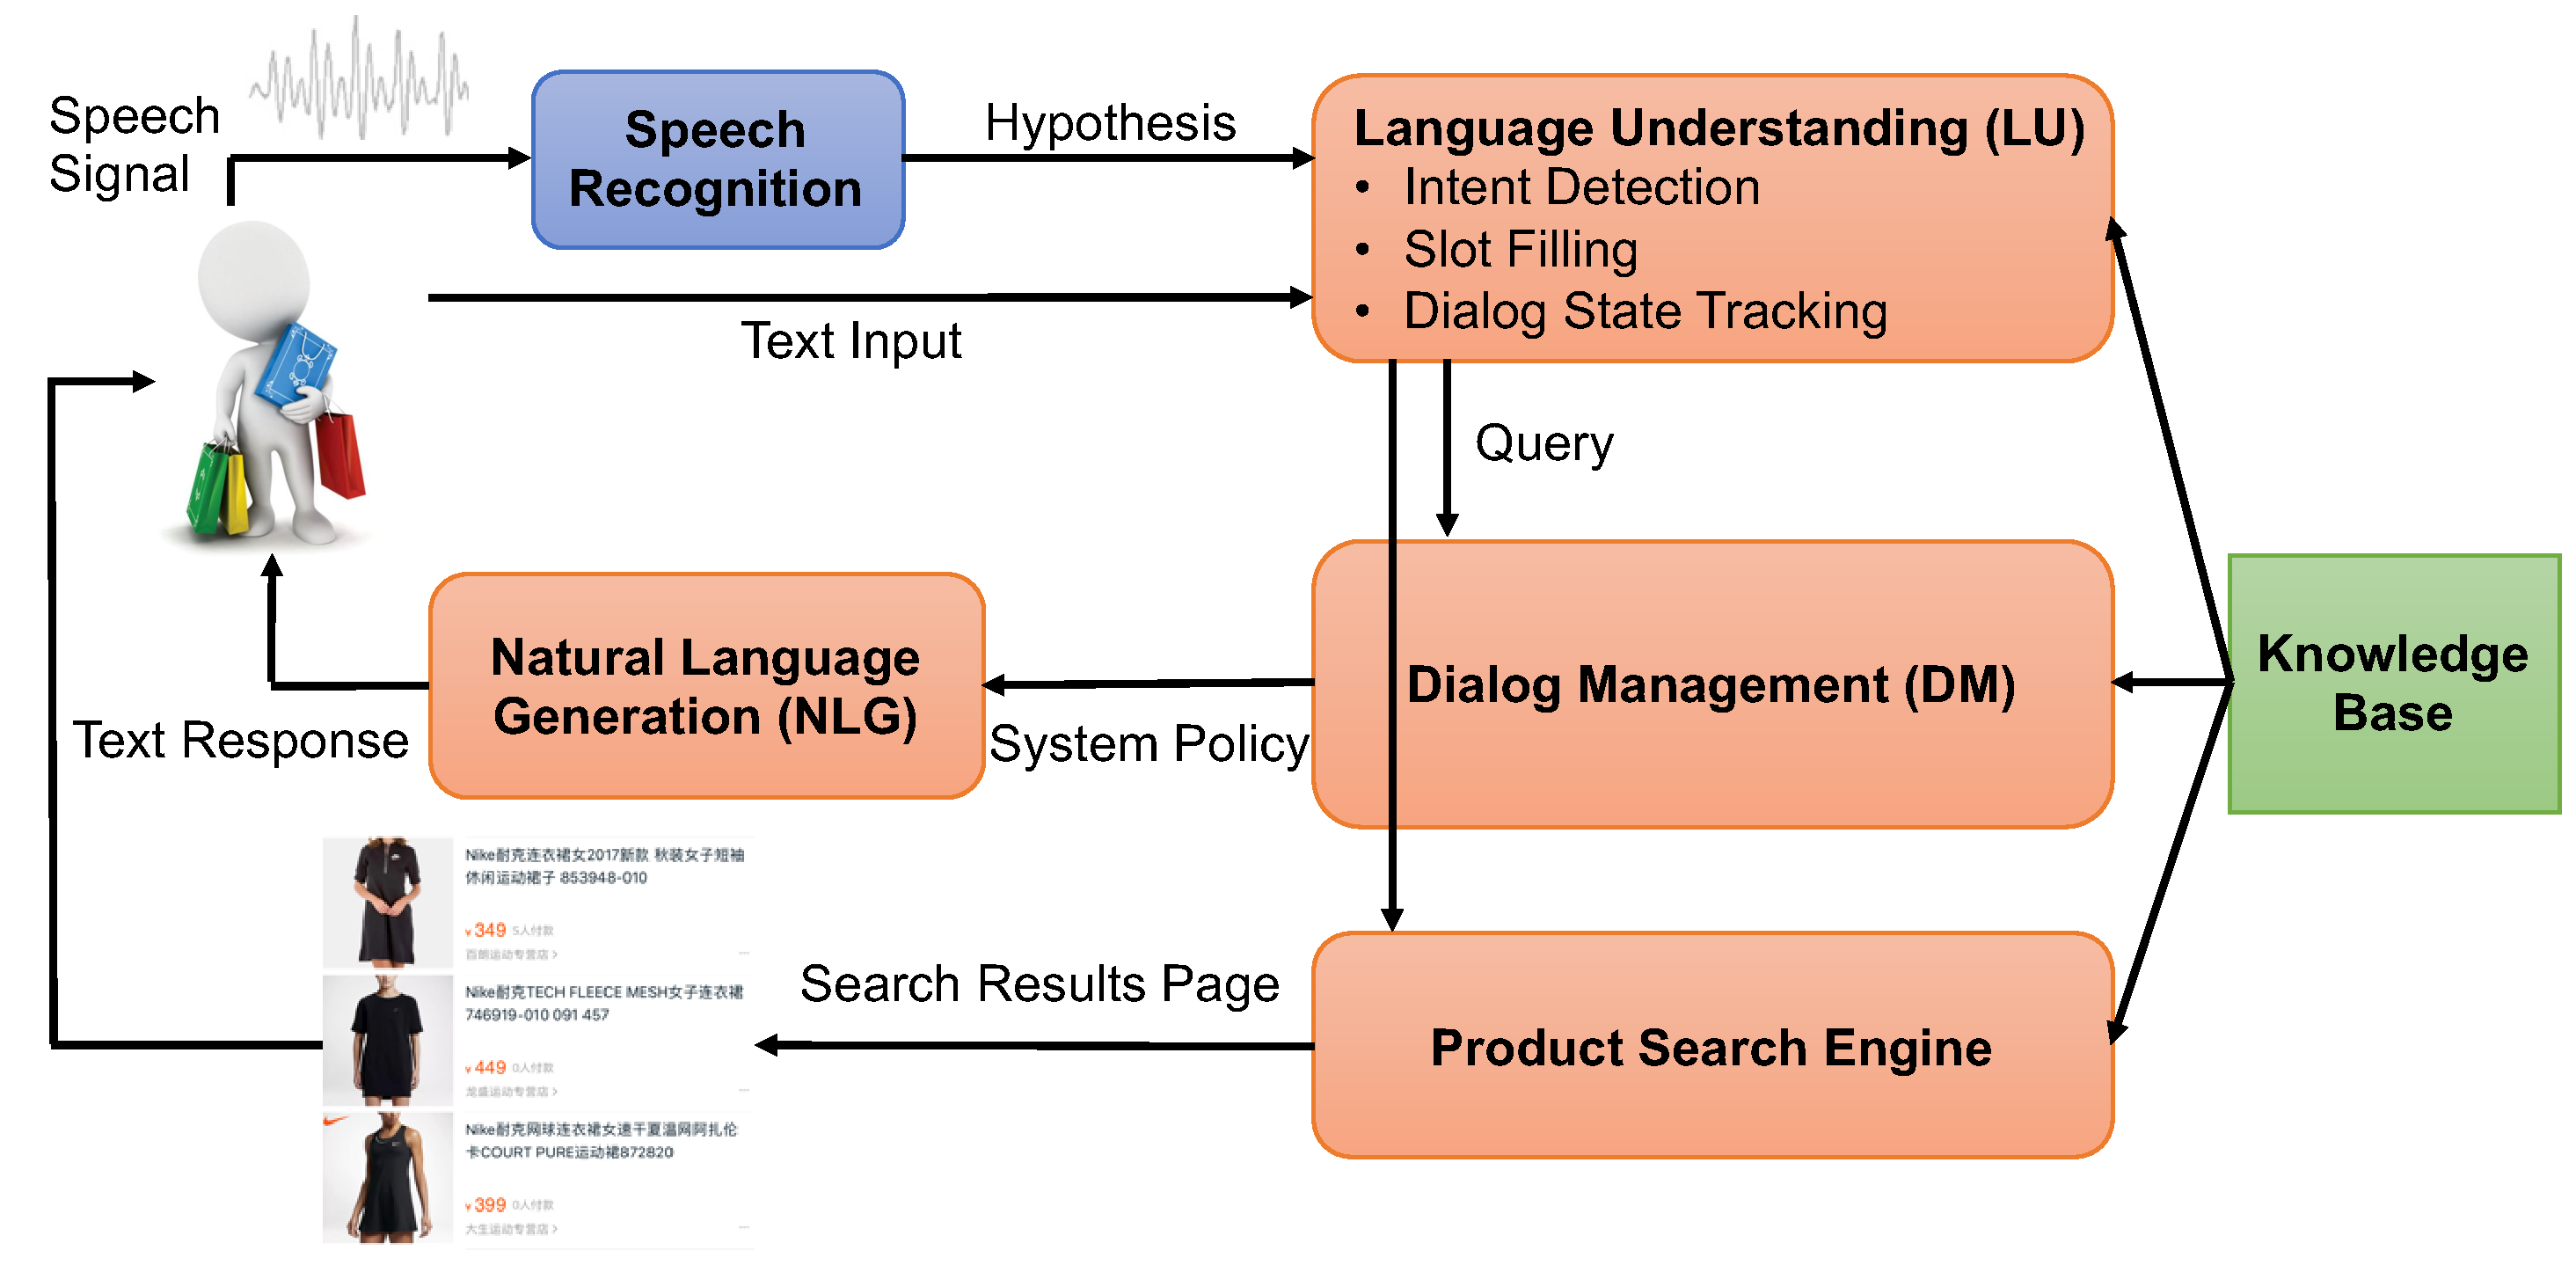
\epsfig{file=figures/dialog_system.eps, width=1.0\columnwidth}
%	\caption{Pipeline framework of task-oriented dialog system for 
%		shopping assistant.}
%	\label{fig:dialog-system}
%	\vspace{-10pt}
%\end{figure}
%\KZ{You need to explain what's slot filling using a very simple and 
%intuitive example. And then you say what's so special about slot filling
%for e-commerce dialogue systems, using some additional examples.}
Slot filling, a sub-problem of NLU, extracts semantic constituents
by using the words of input utterance to fill in pre-defined slots in 
a semantic frame \cite{mesnil2015using}.
%\KZ{Commonly used slots for e-commerce includes ...} 
%\yu{这个句子很跳跃,突然开始讲这个。需要更好的衔接}

In the case of E-commerce shopping, 
there are three named entity types: 
\emph{Category}, \emph{Property Key} and \emph{Property Value}, according to typical E-commerce knowledge base such as the one in \figref{fig:kg}.
We show a real example in \tabref{tab:slot-filling-demo}
with In/Out/Begin (\textbf{I/O/B}) scheme.
In the named entity level,
``dress'' is a Category (\textbf{CG}),
while ``brand'' is labeled as Property Key (\textbf{PK}),
which is the name of one product property.
``Nike'' and ``black'' are labeled as Property Value (\textbf{PV}) since they 
are concrete property values.
However, merely labeling as Property Value is not sufficient as
the shopping assistant needs more fine-grained semantics.
Therefore, in the Slot Filling level, 
we further label ``Nike'' as Brand Property (\textbf{Brand}), 
and ``black'' as Color Property (\textbf{Color}).
In \tabref{tab:slot-filling-demo}, \textbf{B-CG} refers to 
Begin-Category (the meaning of other labels can also be inferred). 
In the meantime, other words in the example utterance that carry no semantic meaning are assigned \textbf{O} label.
\begin{figure}[th]
	\centering
	\epsfig{file=figures/kg2.eps, width=0.7\columnwidth}
	\caption{Structure of E-commerce knowledge-base.}
	\label{fig:kg}
	%\vspace{-10pt}
\end{figure}
%\begin{CJK}{UTF8}{gbsn}
\begin{table*}[h]
	\centering
	\scriptsize
	\begin{tabular}{c|c|c|c|c|c|c|c|c|c|c|c|c|c}
		\toprule
		\multirow{2}{*}{Utterance} & 
\includegraphics[height=1.8\fontcharht\font`\B]{figures/wo.png} & 
\includegraphics[height=1.8\fontcharht\font`\B]{figures/xiang.png} & 
\includegraphics[height=1.8\fontcharht\font`\B]{figures/mai.png} & 
\includegraphics[height=1.8\fontcharht\font`\B]{figures/nai.png} & 
		
\includegraphics[height=1.8\fontcharht\font`\B]{figures/ke.png} & 
\includegraphics[height=1.8\fontcharht\font`\B]{figures/pin.png} & 
\includegraphics[height=1.8\fontcharht\font`\B]{figures/pai.png} & 
		
\includegraphics[height=1.8\fontcharht\font`\B]{figures/de.png} & 
		
\includegraphics[height=1.8\fontcharht\font`\B]{figures/hei.png} & 
\includegraphics[height=1.8\fontcharht\font`\B]{figures/se.png} & 
\includegraphics[height=1.8\fontcharht\font`\B]{figures/lian.png} & 
\includegraphics[height=1.8\fontcharht\font`\B]{figures/yi.png} & 
\includegraphics[height=1.8\fontcharht\font`\B]{figures/qun.png} \\
		\cmidrule{2-14}
		& I & want & buy & \multicolumn{2}{c|}{Nike} & \multicolumn{2}{c|}{brand} & $\backslash$  & \multicolumn{2}{c|}{black} & \multicolumn{3}{c}{dress} \\
		\midrule
		Slot Label & \textbf{O} & \textbf{O} & \textbf{O} & \textbf{B-Brand} & \textbf{I-Brand} & \textbf{B-PK} & \textbf{I-PK} & \textbf{O} & \textbf{B-Color} & \textbf{I-Color} & \textbf{B-CG} & \textbf{I-CG} & \textbf{I-CG} \\
		\midrule
		Named Entity Label & \textbf{O} & \textbf{O} & \textbf{O} & \textbf{B-PV} & \textbf{I-PV} & \textbf{B-PK} & \textbf{I-PK} & \textbf{O} & \textbf{B-PV} & \textbf{I-PV} & \textbf{B-CG} & \textbf{I-CG} & \textbf{I-CG} \\
		\midrule
		Segment Label & \textbf{O} & \textbf{O} & \textbf{O} & \textbf{B} & \textbf{I} & \textbf{B} & \textbf{I} & \textbf{O} & \textbf{B} & \textbf{I} & \textbf{B} & \textbf{I} & \textbf{I} \\
		\bottomrule
	\end{tabular}
	\caption{A real example of slot filling in online shopping scenario.}
	\label{tab:slot-filling-demo}
	%\vspace{-10pt}
\end{table*}
%\end{CJK}
%\yu{What the limits of traditional sequence labeling models for slot filling problem?}

Traditionally, slot filling problem  can be regarded as a sequence 
labeling task,
which assigns an appropriate semantic label to each word in
the given input utterance.
State-of-the-art sequence labeling models are typically based on 
BiLSTM-CRF \cite{huang2015bidirectional,reimers2017optimal}
and evaluated on a commonly used standard dataset ATIS \cite{price1990evaluation} in the slot filling area.
%\KZ{I don't think you need to mention the ATIS dataset here.
%Instead, you should say why the traditional methods don't work
%for the e-commerce slot filling, and in particular, for
%the Chinese language due to word segmentation challenges, etc.
%You should only mention your own
%dataset in the bullets of the contribution below. We are selling our
%approach here, not the dataset. The whole thing from here up to the contribution
%bullets can be shortened quite signficantly. It's too verbose now.}
This dataset is about airline travel in the United States.
%and \tabref{tab:slot-filling-demo-atis} shows an example utterance.
However, the vocabulary size of ATIS is small (only 572)
and slot labels are not diverse enough (mostly related to only time and location)
since airline travel is a relatively small and specific domain,
such that recent deep learning models can achieve very high F1 scores
(nearly 0.96). Recently, a detailed quantitative and qualitative study of this dataset comes to the same conclusion that slot filling models should be tested on a much more real and complex dataset \cite{bechet2018atis}. 

%\begin{table}[h]
%	\centering
%	\scriptsize
%	\caption{An example utterance from the ATIS dataset.}
%	\begin{tabular}{c|c}
%		\toprule
%		Utterance & flights $|$ from $|$ Dallas $|$ to $|$ New $|$ York \\
%		\midrule
%		Slot Label & \makecell{\textbf{O} $|$ \textbf{O} $|$ \textbf{B-fromloc.city\_name} $|$ \textbf{O} $|$ \textbf{B-toloc.city\_name} $|$ \\ \textbf{I-toloc.city\_name}}  \\
%		\bottomrule
%	\end{tabular}
%	\label{tab:slot-filling-demo-atis}
%	\vspace{-10pt}
%\end{table}

%\KZ{I think we need to justify a bit more strongly why we need this
%new dataset.}
%\yu{In this work, we are tackling the real-world problem of slot filling for a shopping assistant on Taobao which is the largest Chinese E-commerce platform in the world.
%	It's the first attempt in the existing research for both academic and industry without any of the similar dataset.
%}

In this paper, we try to tackle a real-world slot filling problem 
for one of the largest E-commerce platform in China.
The semantic slots are much more diverse and informative than ATIS.
%Thus, we create another bigger, more complex dataset
%in the domain of Chinese E-commerce shopping 
%assistant~\footnote{This dataset is available at \url{http://will.release.after.accepted}.}.
%This dataset comes from a real world application 
%and increases the difficulty for slot filling.
%This dataset comes from a real world application and the
%semantic slots are more diverse and informative than ATIS, 
%which increases the difficulty for the task.
%For example, there are 26 semantic labels in the Dress category,
%which describe different properties for a dress such as color, brand and style, while most semantic labels of ATIS 
%are related to only time and location.
For example, to describe different properties of a product for 
the purpose of utterance understanding,
we define large amount of informative slot labels such as color, brand, 
style, season, gender and so on.
In contrast, most semantic labels of ATIS are related to only time and location.
Furthermore, the Chinese language used for e-commerce is more complex 
and the semantically rich expressions make it harder to understand.
%\yu{For example, only in dress domain, there are 1265 Chinese characters, and the amount of segmented terms can be much larger.}
%\yu{If we delete the following examples.}
%For example, ``红色'' and ``红'' both mean red, ``品牌'' and ``牌子'' both mean brand, ``耐克'' and ``Nike'' and ``Niky'' all mean Nike.
Whereas in ATIS, 
%\yu{there are only 572 words,}
expression can be simpler, and most expressions are standard locations or time.
Thus, large scale semantic slots and more complex expressions bring problem such as data sparsity.
Traditional end-to-end sequence labeling model may not be able to handle it.

Besides, Chinese language, like many other Asian languages, is not
word segmented by nature, and word segmentation is a difficult
first step in many NLP tasks.
Without proper word segmentation, sequence labeling becomes very challenging
as the errors from segmentation will propagate.
On the other hand, more than 97\% of the chunks in ATIS data 
have only one or two words,
in which segmentation (or chunking) is not a serious problem.
Due to these reasons,
if we simply apply basic sequence labeling models,
which can be regarded as an end-to-end method,
%on the Chinese E-commerce dataset,
the sentences may not be segmented correctly in the first place.
%\KZ{We need to stress more why the existing LSTM-CRF models can't handle
%the chinese e-commerce dataset.}
%\yu{Our focus and point is multi-task.}
Then the errors will propagate and the resulting slot labels will be incorrect.

%4. How Deep Cascade Multi-task learning works and the performance?
%In this paper, we employ the idea of multi-task learning
%to tackle slot filling task in Chinese E-commerce.
%\KZ{I think the EC KB is part of your solution, not part of the problem.
%You problem is understand user utterance. So you can't use the structure
%of KB as your motivation. Other ppl will say, then why don't you use another
%kind of KB?}
%\xusheng{Emphases more on e-Commerce KB?}
%\yu{你把使用multi-task的动机放在这句话的之后讲的。考虑能不能倒过来,先讲几个task其实能相互帮助,再说提出一个多任务的模型来做。}
In this paper, we propose to employ multi-task sequence labeling model
to tackle slot filling in a novel Chinese E-commerce dialog system.
Inspired by the natural structure of E-commerce knowledge base shown in \figref{fig:kg},
we extract two additional lower-level tasks from the slot filling task: 
{\em named entity tagging} and {\em segment tagging}.
Example labels of these two tasks 
are shown in the bottom two rows of \tabref{tab:slot-filling-demo}.
Segment tagging and named entity tagging can be regarded as 
syntactic labeling, 
while slot filling is more like semantic labeling.
%\yu{Talk more about multi-task learning?}
With the help of information sharing ability of multi-task learning,
once we learn the information of syntactic structure of an input sentence,
filling the semantic labels becomes much easier.
Compared to directly attacking slot filling,
these two low-level tasks are much easier to solve
due to fewer labels.
To this end, we propose a Deep Cascade Multi-task Learning model,
and co-train three tasks in the same framework
with a goal of optimizing the target slot filling task.
%\KZ{Earlier you said two tasks, now suddenly three tasks...}
%5. Contribution and Conclusion.

The contributions of this paper are summarized below:
\begin{itemize}
	%\itemsep0em
	\item To the best of our knowledge, this is the first piece of work focusing on slot filling in E-commerce. 
	We propose a novel deep multi-task 
	sequence labeling model (DCMTL) with cascading and 
	residual connection to solve it (\secref{sec:dcmtl}).
	\item We develop a Chinese E-commerce shopping assistant dataset 
	ECSA (\secref{sec:data}), which is much bigger and different from 
	the common ATIS dataset, and would be a valuable contribution to 
	dialog system research.  
	%We believe this dataset will contribute more to the future 
	%research of dialog natural language understanding.
	\item We evaluate DCMTL in both offline and online settings.
	Offline results show the model outperforms 
	several strong baseline methods by a substantial margin of $14.6\%$ on $F1$ score (\secref{sec:eval}).
	Online testing deployed on the mentioned E-commerce platform shows that 
	slot filling results returned by our model achieve 130\% improvement 
	on accuracy which significantly benefits to the understanding of users' utterances (\secref{sec:case_study}).
	Our model has already gone production in the platform.
	%\KZ{Can we say something about the
%actual commercial impact? The accuracy seems illusive. How can you measure
%accuracy in real world interaction with users?}
%	\yu{There is no directly commercial impact, slot filling is a basic module for Query Rewrite in search area and Dialog State Tracking in dialog area.
%		So it's performance can significantly affect the user experience of the searching results. 
%	}
\end{itemize}

%The rest of the paper is organized as follows:
%\secref{sec:problem} provides the formal definition of slot filling problem in our study.
%\secref{sec:model} describes the proposed multi-task sequence labeling architecture.
%\secref{sec:data} introduces the traditional ATIS dataset and how we collect our ECSA dataset.
%Then \secref{sec:implementation} gives the implementation details of our model for reproducibility.
%\secref{sec:eval} presents the experimental results and analysis both on ATIS and ECSA data.
%We include the detailed comparison with baseline models, ablation test for model analysis, online case study and evaluation.
%\secref{sec:related} discusses some related work.
%Finally \secref{sec:conclusion} concludes the paper and points out some 
%future research directions.
